\documentclass[11  pt]{exam} 
\usepackage[lmargin=1in,rmargin=1.75in,bmargin=1in,tmargin=1in]{geometry}  


% For hyperlinking everything
\usepackage{hyperref}
\hypersetup{
	colorlinks=true, %set true if you want colored links
	linktoc=all,     %set to all if you want both sections and subsections linked
	linkcolor=blue,  %choose some color if you want links to stand out
}


\usepackage[latin1]{inputenc}
\usepackage{amsmath}
\usepackage{mathrsfs}  
\usepackage{amsfonts}
\usepackage{amssymb}
\usepackage{graphicx}
\usepackage{subfig}
\usepackage{caption}
\usepackage{algorithm}
%\usepackage{algcompatible}
%\usepackage{algorithmicx}
\usepackage{algpseudocode}

\usepackage{titlesec}
\titleformat{\section}{\fontfamily{lmss}\fontsize{14}{15}\bfseries}{\thesection}{1em}{}
\titleformat{\subsection}{\fontfamily{lmss}\fontsize{12}{15}\bfseries}{\thesubsection}{1em}{}




\usepackage{amsthm}

\newtheoremstyle{noit}
{10pt}% <Space above>
{10pt}% <Space below>
{}% <Body font>
{}% <Indent amount>
{\bfseries}% <Theorem head font>
{.}% <Punctuation after theorem head>
{.5em}% <Space after theorem headi>
{}% <Theorem head spec (can be left empty, meaning `normal')>

\newtheoremstyle{example}
{10pt}% <Space above>
{10pt}% <Space below>
{}% <Body font>
{20pt}% <Indent amount>
{\bfseries}% <Theorem head font>
{.}% <Punctuation after theorem head>
{.5em}% <Space after theorem headi>
{}% <Theorem head spec (can be left empty, meaning `normal')>


\newtheoremstyle{indented}{20pt}{20pt}{\addtolength{\leftskip}{2.5em}}{}{\bfseries}{.}{.5em}{}


\newtheorem{theorem}{Theorem}
\numberwithin{theorem}{section}
\newtheorem{lemma}[theorem]{Lemma}
\newtheorem{corollary}[theorem]{Corollary}
\newtheorem{observation}{Observation}
%\numberwithin{observation}{section}
%\numberwithin{definition}{section}
\newtheorem{conjecture}{Conjecture}
\newtheorem{Qu}{Question}
\newcommand{\QU}{\begin{Qu}\normalfont}

\theoremstyle{noit}
\newtheorem{fact}{Fact}
\newtheorem{definition}{Definition}

\theoremstyle{indented}
\newtheorem{example}{Example}

\theoremstyle{indented}
\newtheorem{problem}{Problem}


%\newenvironment{proof}{\noindent{\bf Proof:} \hspace*{1em}}{
%    \hspace*{\fill} $\Box$ }
%\newenvironment{proof_of}[1]{\noindent {\bf Proof of #1:}
%    \hspace*{1em} }{\hspace*{\fill} $\Box$ }
%\newenvironment{proof_claim}{\begin{quotation} \noindent}{
%    \hspace*{\fill} $\diamond$ \end{quotation}}
\newcommand{\vs}[1]{\vspace{#1}}

\newcommand{\lecture}[2]{
 \noindent
\begin{center}
	\framebox{
		\vbox{
			\hbox to 5.78in { {\bf CSCE 411: Design and Analysis of Algorithms (Honors)} \hfill  }
			\vspace{2mm}
			\hbox to 5.78in { {\Large \hfill Lecture #1\hfill} }
			\vspace{2mm}
			\hbox to 5.78in { {\it Date: #2 \hfill Samson Zhou} }
		}
	}
\end{center}
\vspace*{4mm}
}

\newcommand{\week}[2]{
 \noindent
\begin{center}
	\framebox{
		\vbox{
			\hbox to 5.78in { {\bf CSCE 411: Design and Analysis of Algorithms (Honors)} \hfill  }
			\vspace{2mm}
			\hbox to 5.78in { {\Large \hfill Week #1\hfill} }
			\vspace{2mm}
			\hbox to 5.78in { {\it Date: #2 \hfill Nate Veldt, updated by Samson Zhou} }
		}
	}
\end{center}
\vspace*{4mm}
}

\newcommand{\sweek}[2]{
 \noindent
\begin{center}
	\framebox{
		\vbox{
			\hbox to 5.78in { {\bf CSCE 411: Design and Analysis of Algorithms (Honors)} \hfill  }
			\vspace{2mm}
			\hbox to 5.78in { {\Large \hfill Week #1\hfill} }
			\vspace{2mm}
			\hbox to 5.78in { {\it Date: #2 \hfill Samson Zhou} }
		}
	}
\end{center}
\vspace*{4mm}
}

\newcommand{\hw}[2]{
	\noindent
	\begin{center}
		\framebox{
			\vbox{
				\hbox to 5.78in { {\bf CSCE 411: Design and Analysis of Algorithms} \hfill  }
				\vspace{2mm}
				\hbox to 5.78in { {\Large \hfill Homework #1\hfill} }
				\vspace{2mm}
				\hbox to 5.78in { {\it Due date: #2 \hfil} }
			}
		}
	\end{center}
	\vspace*{4mm}
}



\newcommand{\under}[1]{\underline{\hspace{#1}}}
\setlength{\parindent}{0em}

%\usepackage[tagged]{accessibility}

% Graph terms
\newcommand{\vol}{\textbf{vol}}
\newcommand{\cut}{\textbf{cut}}


% Matrices
\newcommand{\mA}{\textbf{A}}
\newcommand{\mB}{\textbf{B}}

% vectors
\newcommand{\ve}{\textbf{e}}
\newcommand{\vx}{\textbf{x}}


% Other
\newcommand{\calN}{\mathcal{N}}

\usepackage{mathtools}
\DeclarePairedDelimiter\ceil{\lceil}{\rceil}
\DeclarePairedDelimiter\floor{\lfloor}{\rfloor}


\newcommand*{\aitem}{ \item[{
\includegraphics[width=0.8cm,height=0.5cm]{figures/A}} ]  }
\newcommand*{\bitem}{ \item[{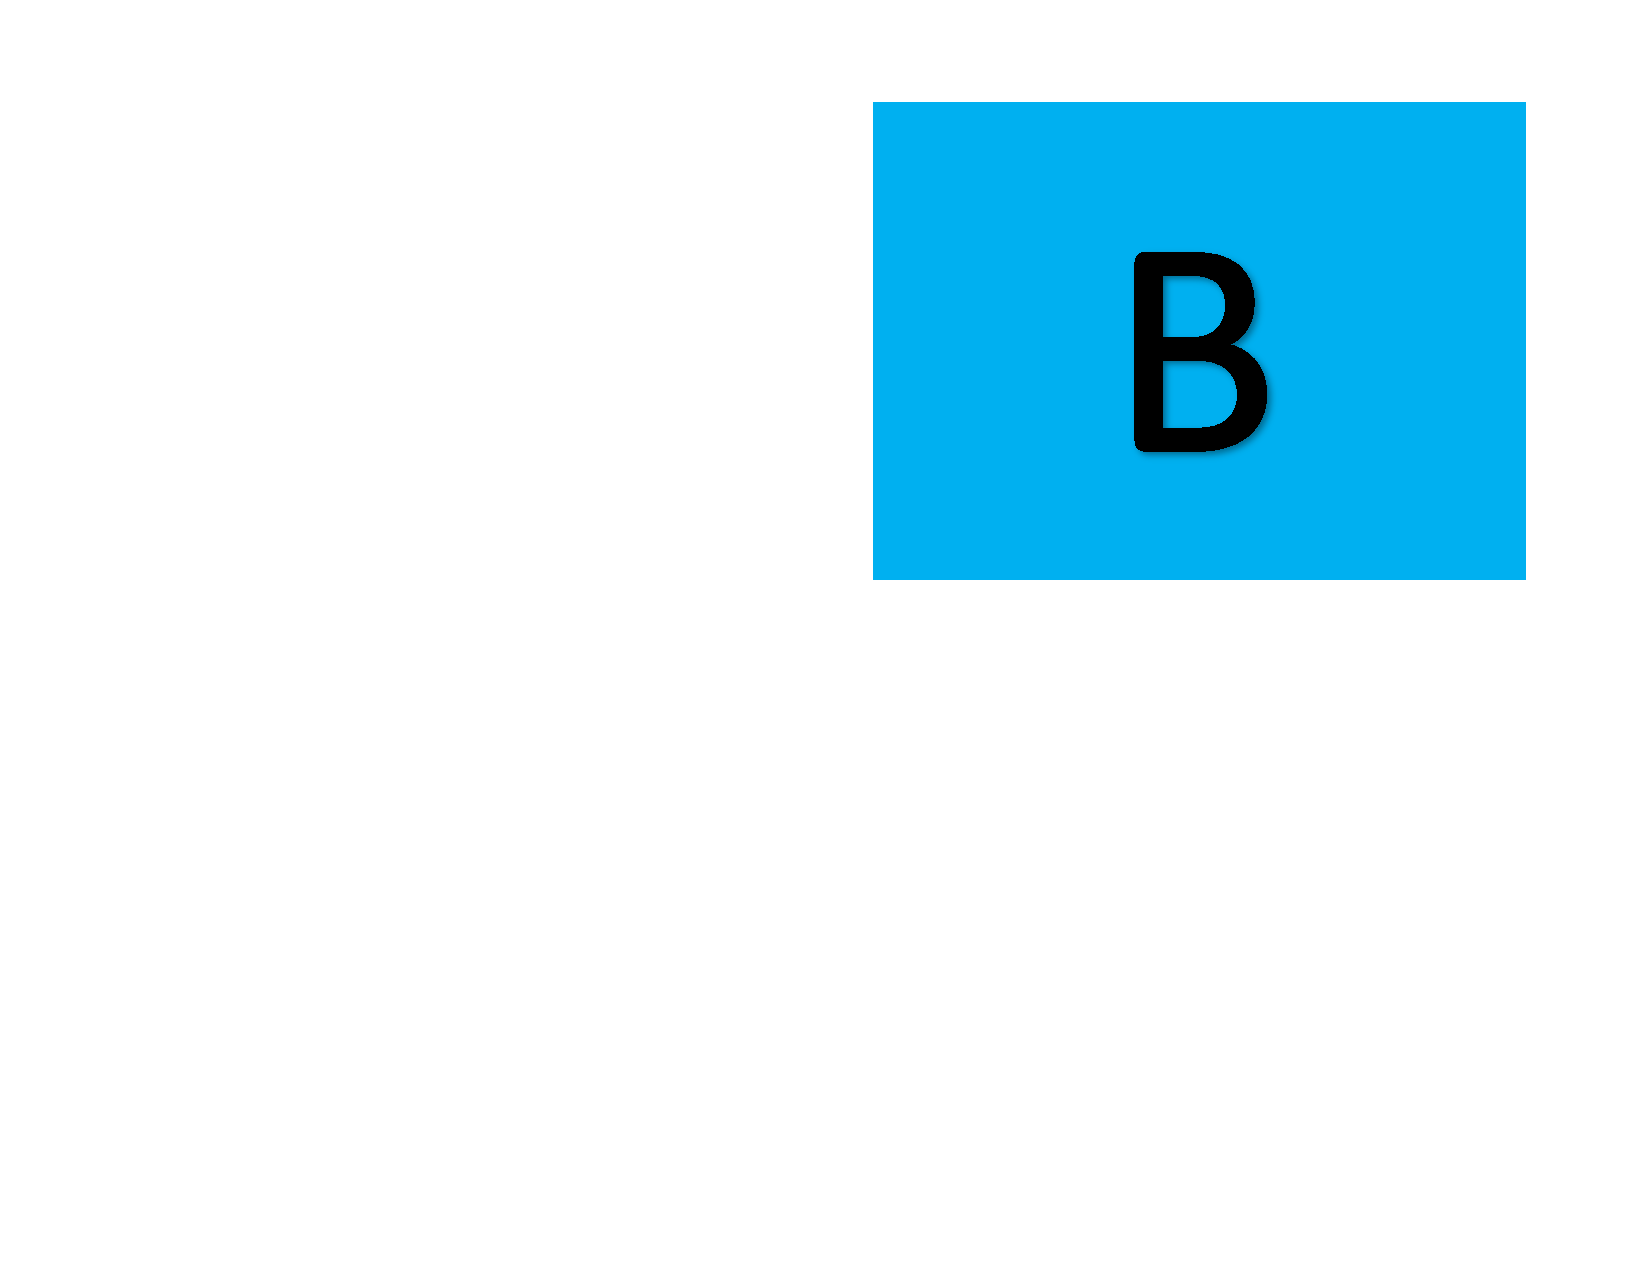
\includegraphics[width=0.8cm,height=0.5cm]{figures/B}} ]  }
\newcommand*{\citem}{ \item[{
\includegraphics[width=0.8cm,height=0.5cm]{figures/C}} ]  }
\newcommand*{\ditem}{ \item[{
\includegraphics[width=0.8cm,height=0.5cm]{figures/D}} ]  }
\newcommand*{\eitem}{ \item[{
\includegraphics[width=0.8cm,height=0.5cm]{figures/E}} ]  }
\newcommand*{\fitem}{ \item[{
\includegraphics[width=0.8cm,height=0.5cm]{figures/F}} ]  }


\newcommand{\hide}[1]{\underline{\phantom{#1 #1}}}

\usepackage{setspace}

\onehalfspacing

\begin{document}
	
	
	\week{7, Exam 2 Review}{October 15, 2026}
	
	%	\paragraph{Course Logistics}	
	%	\begin{itemize}
	%		\item First test is this Friday
	%	\end{itemize}
	
	\section{Test format and instructions}
	
	\begin{itemize}
		\item Some multiple choice questions, some long answer questions
		\item You do not need to prove something unless you are explicitly asked to prove something
		\item You may be asked to explicitly prove something 
		\item Scratch paper will be provided
		\item No calculators or electronic devices. You will not need them. If you have to do any computations, they will be basic enough to do by hand. 
		\item You will put your name on the front page, and put your initials at the top of every other page.
	\end{itemize}
	
%	{\Large  \centering This is all the same as Test 1!}
	
	A few other notes:
	\begin{itemize}
		\item If something was on a homework or in a lecture, it could be on the test.
		\item Some questions may involve a combination of a couple different things we've seen in different lectures.
		\item If we covered a proof of a result, you can reference it as fact without re-proving it, unless the question specifically is asking you to provide proof details.
	\end{itemize}
	
	\newpage 
	
	\section{Topics Covered on the Test}
	
	%	These notes go over the main topics we have studied, list questions for you to fill in that you should know about on the test, and give some examples of things you might be required to do on the test.
	%	
	\subsection{Summary of the summary}
	\begin{itemize}
		\item Graph basics (adjacency matrix, adjacency list, directed/undirected, weighted/unweighted, cyclic/acyclic)
		\item (BFS) Breadth-first search
		\item (DFS) Depth-first search
		\item (SSSP) Single source shortest paths (Bellman-Ford, Dijkstra's)
		\item Maximum $s$-$t$ flow and minimum $s$-$t$ cut (Ford-Fulkerson, Edmonds-Karp)
		\item Linear programming, duality
		\item Continuous optimization (Convexity, smoothness, gradient descent)
		\end{itemize}

For all of the graph algorithms, here's the short answer on what you should know:

\begin{itemize}
	\item How is the problem defined? In particular, what type of graph does it apply to? Are there restrictions?
	\item What algorithms solve the problem, what is their basic mechanism, and their runtime?
	\item Don't just know how to eye-ball a solution for a small graph. You should know the mechanics of each algorithm well enough that you could apply it to a small graph, could write out pseudocode if need be, and provide a runtime analysis 
\end{itemize}
	
\subsection{Graph Basics}
	
	\begin{itemize}
		\item Representing a graph as a list or a matrix
		\item Undirected and directed, weighted and unweighted (which of these can be viewed as special cases of others?)
		\item Strongly connected and weakly connected components. What is their relation? How are they defined?
		\item What is a bipartite graph?
	\end{itemize}

	\subsection{Breadth first search specifics}

	\begin{itemize}	
		\item Running a BFS on a weighted graph just means ignore the edge weights. (You wouldn't say ``BFS doesn't apply if the graph is weighted.'')
		\item Remember what a breadth-first tree is and how to find it.
		\item Make sure you know the runtime
	\end{itemize}


	\subsection{Depth-first search}
		\begin{itemize}	
			\item Know the different edge types in a depth-first search and what they mean
			\item Know the two main applications we discussed in class and how to use DFS for them.
		\end{itemize}

	%\subsection{Minimum Spanning Tree}
%\begin{itemize}	
	%\item You should know the basic mechanism behind both Prim's and Kruskal's algorithm
	%\item You should know what a cut is, and what a ``safe'' edge is.
	%%\item We did a mini runtime analysis for Prim's algorithm: you should know what the runtime is and how that basic argument worked (there are many other algorithms with similar types of runtime analyses).
%\end{itemize}

	\subsection{Single source shortest paths algorithm}

\begin{itemize}	
	\item Two algorithms we saw: Bellman-Ford, Dijkstra's %(and we talked about two ways to implement the min-priority queue).
	\item You should understand the basic mechanism behind each, and different pros/cons of their runtimes
\end{itemize}

	\subsection{Min-cut Max-Flow Problem and algorithms}

	\begin{itemize}	
		\item What is the definition of an $s$-$t$ flow function? What is an $s$-$t$ cut in a directed graph?
		\item What is the basic idea behind the algorithms we have seen? Hint: it isn't that you repeatedly try to send flow from $s$ to $t$ as long as you can find unsaturated paths in the original graph $G$. 
		\item What is an augmenting path and a residual graph? 
		\item What is the basic mechanism behind Ford-Fulkerson? What's its runtime and why?
		\item What is the difference between Ford-Fulkerson and Edmonds-Karp? What is the runtime difference? 
		\item You would not be expected to reproduce a long proof such as the one we did for Edmond's Karp, but you might be expected to understand/explain one small subset.
		\item You should know that what the maximum-flow minimum-cut theorem says and how to use it to verify that a flow or cut is optimal or not optimal.
	\end{itemize}
	
	
	\subsection{Linear programming and duality}
	\begin{itemize}

		\item What is a linear program? Identify its decision variables, objective function, and constraints.
		\item How do you formulate a word problem as a linear program? You should be able to explain what each variable and constraint represents.
		\item What does it mean for a solution to be feasible or optimal? What does it mean for a linear program to be infeasible or unbounded?
		\item What does the feasible region look like geometrically? You should be able to solve a small linear program with two variables by drawing its constraints and comparing objective values.
		\item Given a primal linear program, how do you write its dual?	Pay attention to the directions of inequalities and restrictions on the signs of variables.
		\item What does weak duality say? You should understand its proof and explain where primal and dual feasibility are used.
		\item What does strong duality say when the primal has a finite optimal value? How can a primal feasible solution and a dual feasible solution with equal objective values certify that both are optimal?
		\item How is the maximum-flow minimum-cut theorem related to linear programming duality?
	\end{itemize}

	\subsection{Convex optimization and gradient descent}

	\begin{itemize}
		\item What does it mean for a set or a function to be convex? What is the first-order characterization of convexity for a differentiable function?
		\item What is the relationship between local and global minima of a convex function? For differentiable, unconstrained convex minimization, why does a zero gradient certify a global minimum?
		\item What is a gradient, and how do you compute it? How does it relate to the derivative of a function of one variable?
		\item What does it mean for a function to be Lipschitz continuous or smooth? Distinguish a bound on changes in function values, a bound on the gradient itself, and a bound on changes in the gradient.
		\item What is the basic mechanism behind gradient descent? Know the update rule
		\[x_{t+1}=x_t-\eta\,\nabla f(x_t),\]
		where $\eta>0$ is the step size. You should be able to write pseudocode and carry out a few iterations on a simple function.
		\item What role does the step size play? How does smoothness help us choose it, and why can a step size that is too large cause oscillation or divergence?
		\item How does the smoothness inequality show that a suitable gradient descent step decreases the objective when the gradient is nonzero?
		%\item Know the convergence guarantee for gradient descent on a convex, smooth function and the assumptions it requires. How does the number of iterations depend on the smoothness, initial distance to an optimal solution, and desired accuracy? You should be able to use a convergence bound to determine how many iterations suffice for $f(x_T)-f(x^\star)\le\epsilon$.

	\end{itemize}

	\section{Practice Problems}
	
	\begin{questions}
		
		\question When does breadth-first search solve the same problem as Dijkstra's algorithm?
		
		\question What are applications of a breadth first search? What problem(s) does it solve?
		
		\question What are applications for depth first search? What problem(s) does it solve?
					
		\question Write down the adjacency matrix and the adjacency list for each of the sample graphs.
		
		\question Draw the breadth-first tree of the sample graph 1 from starting node $e$
		
		\question Find the minimum $s$-$t$ cut of sample graph 1 when $s = a$ and $t = f$. Explain whether you get the same minimum $s$-$t$ cut value when $s = f$ and $t = a$.
		
		\question Write out a valid $s$-$t$ flow for the graph in Figure 2. 
%		Then write the residual graph for that flow (good exercise to do with a partner---give the residual graph for your partner's flow function).
			
		\question Solve other BFS, DFS, single source shortest path problems on the sample graphs (e.g., try a different source and/or sink node, change weights slightly, etc.)
		
		
		\paragraph{Sample Graphs}
		
		\begin{figure}
			\centering
			\caption{Sample graph 1}
			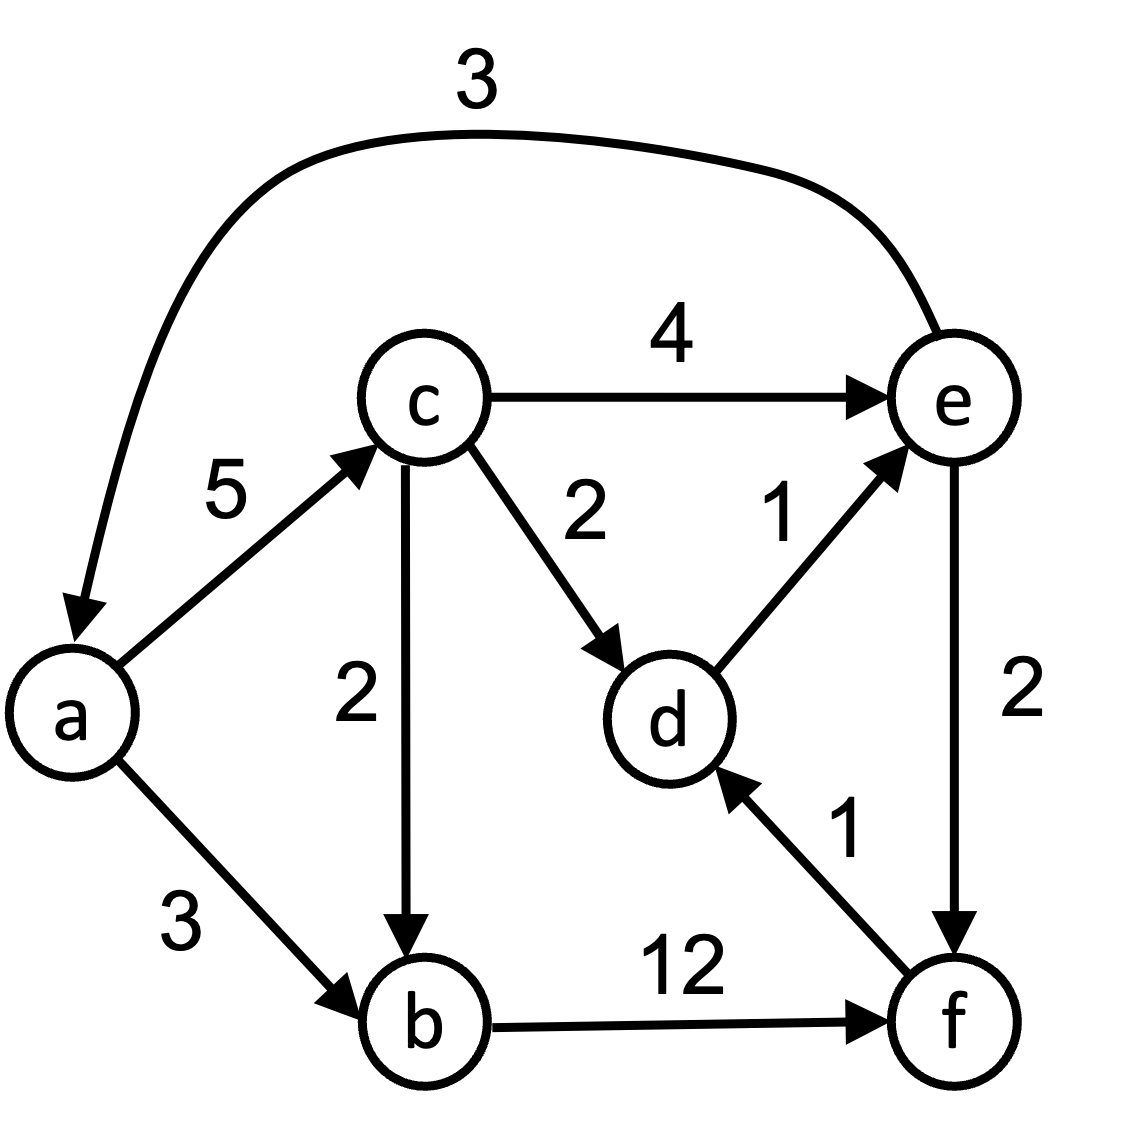
\includegraphics[width = .5\linewidth]{dijkstrasalg}
		\end{figure}
	
	
			\begin{figure}
				\centering
				\caption{Sample graph 2}
				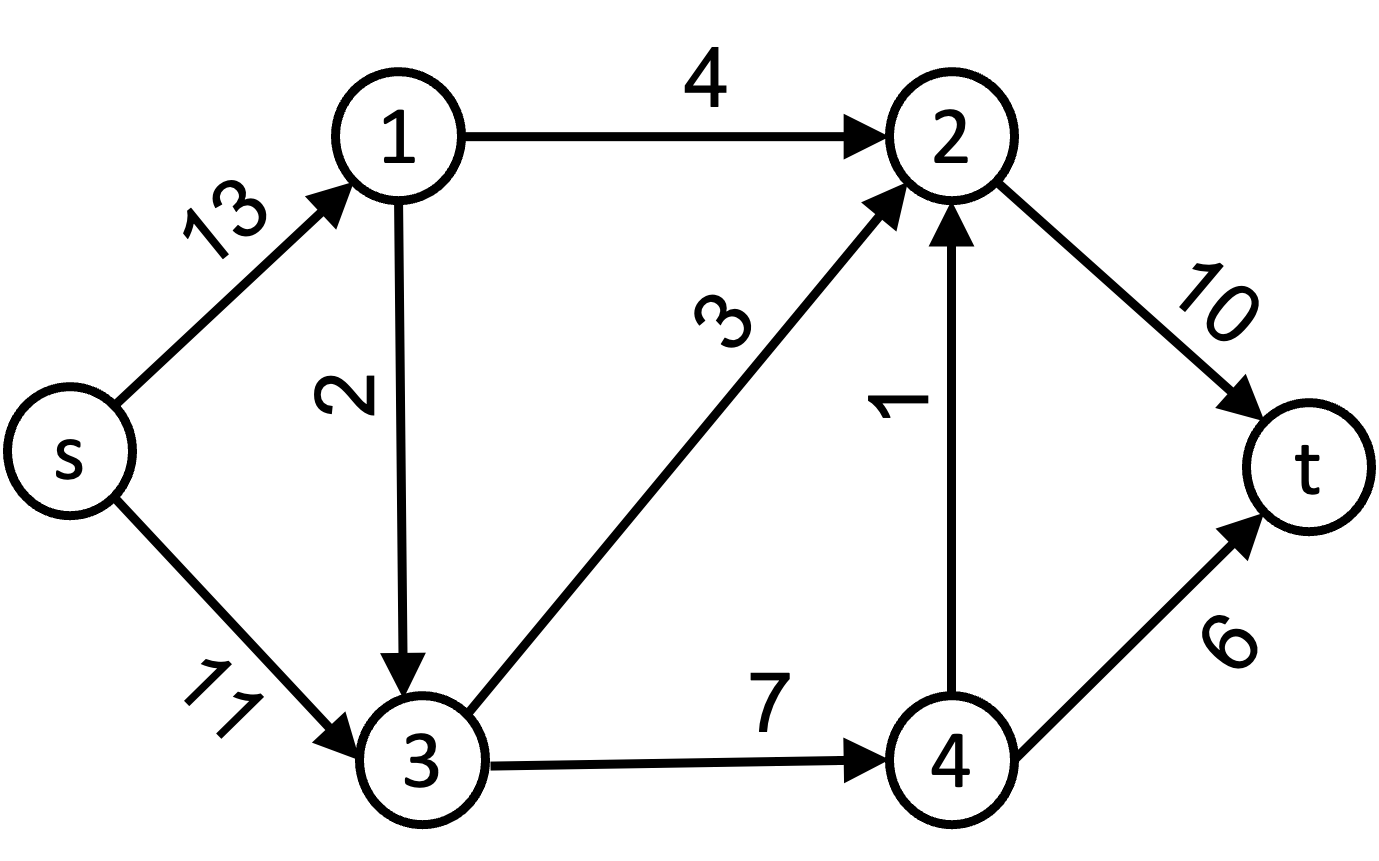
\includegraphics[width = .5\linewidth]{flow1}
			\end{figure}
		
					\begin{figure}
			\centering
			\caption{Sample graph 3}
			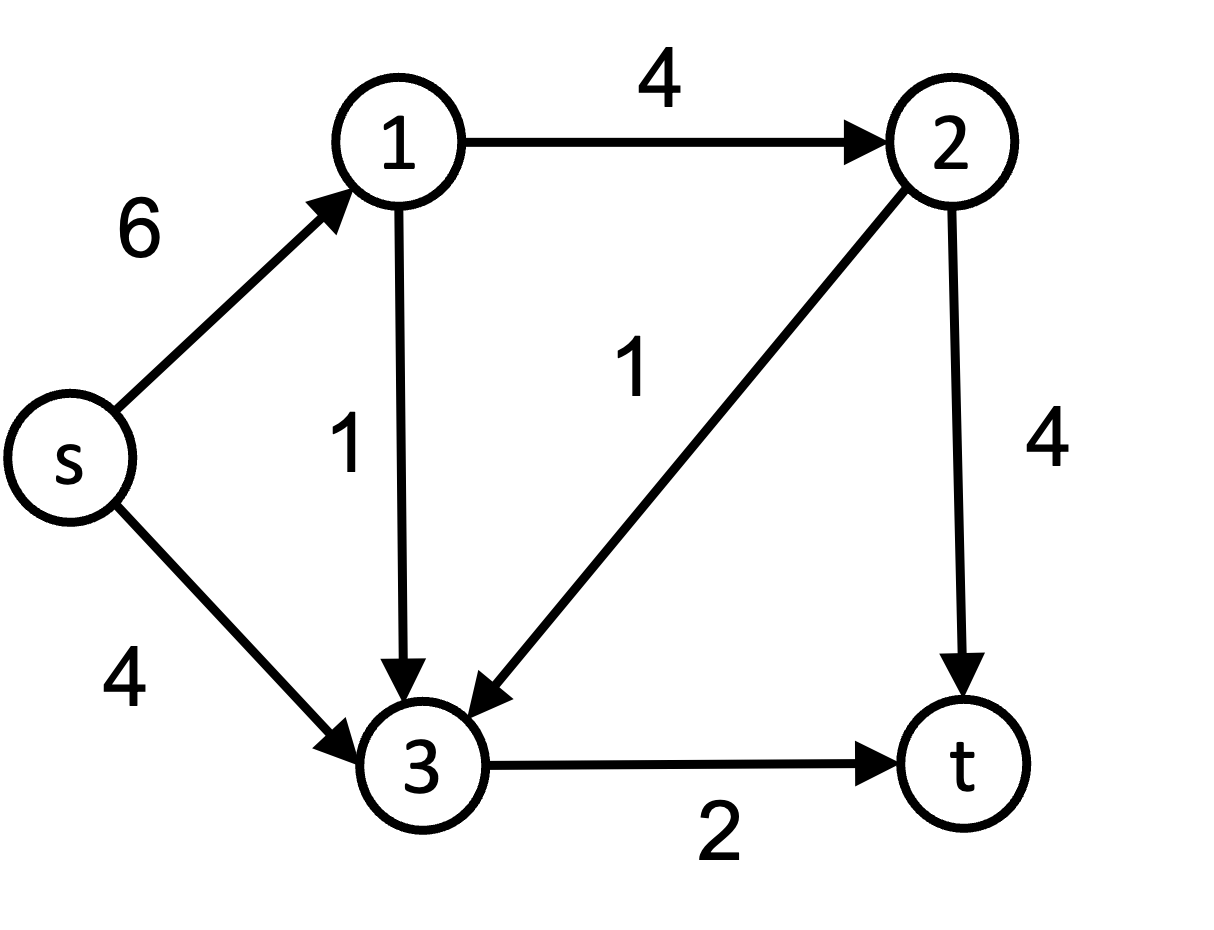
\includegraphics[width = .5\linewidth]{dag1}
		\end{figure}
	
	\clearpage

		\paragraph{Linear programming and duality}



		\question Formulate each of the following problems as a linear program. Clearly define your variables, objective function, and constraints. Amounts may be fractional.

		\begin{parts}

			\part A factory produces chemicals $A$ and $B$. Each unit of $A$ requires two hours on machine 1 and one hour on machine 2, and earns a profit of \$3. Each unit of $B$ requires one hour on each machine and earns a profit of \$2. Machine 1 is available for six hours and machine 2 is available for four hours. Maximize the total profit.

			\part Each unit of food $A$ costs \$3 and provides two units of protein and one unit of fiber. Each unit of food $B$ costs \$3 and provides one unit of protein and two units of fiber. Find a minimum-cost combination providing at least six units of protein and at least six units of fiber.

		\end{parts}



		\question Consider the linear program

		\[
			\begin{array}{ll}
				\text{maximize} & 3x+2y\\
				\text{subject to} & x+y\le 4,\\
				& 2x+y\le 6,\\
				& x,y\ge 0.
			\end{array}
		\]

		\begin{parts}

			\part Draw the feasible region and identify its vertices. Find an optimal solution and its objective value.

			\part Write the dual linear program.

			\part Find a dual feasible solution that certifies your primal solution is optimal. Explain why this is a valid certificate.

		\end{parts}



		\question Consider the primal and dual linear programs

		\[\begin{array}{ll}
				\text{maximize} & c^{\mathsf T}x\\
				\text{subject to} & Ax\le b,\quad x\ge 0
			\end{array}
			\qquad
			\begin{array}{ll}
				\text{minimize} & b^{\mathsf T}y\\
				\text{subject to} & A^{\mathsf T}y\ge c,\quad y\ge 0.
			\end{array}
		\]

		Recall that $y^{\mathsf T}Ax=(A^{\mathsf T}y)^{\mathsf T}x$. Prove that every primal feasible $x$ and dual feasible $y$ satisfy

		\[c^{\mathsf T}x\le b^{\mathsf T}y.\]

		Explain where each feasibility condition is used. Do not invoke strong duality.



		\question Classify each linear program as infeasible, feasible with a finite optimum, or feasible with an unbounded objective. For each feasible program, also determine whether its feasible region is bounded. Justify your answers.

		\begin{parts}

			\part Maximize $x+y$ subject to $x+y\le 1$, $x+y\ge 2$, and $x,y\ge 0$.

			\part Maximize $x+y$ subject to $x-y\le 1$ and $x,y\ge 0$.

			\part Minimize $x+y$ subject to $x+y\ge 1$ and $x,y\ge 0$.

			\part Maximize $x$ subject to $x\le 2$ and $x,y\ge 0$.

		\end{parts}



		\question Let $G=(V,E)$ be a directed graph with source $s$, sink $t$, and nonnegative edge capacities $c_e$.

		\begin{parts}

			\part Formulate maximum $s$-$t$ flow as a linear program. Specify the variables, capacity constraints, flow conservation constraints, and objective function.

			\part Given an $s$-$t$ cut, explain why its capacity is an upper bound on the value of every feasible flow. How can a flow and a cut together certify optimality?

		\end{parts}



		\paragraph{Convex optimization and gradient descent}



		\question Let $f:\mathbb{R}^d\to\mathbb{R}$ be differentiable and convex.

		\begin{parts}

			\part State the first-order inequality that characterizes convexity.

			\part Use this inequality to prove that if $\nabla f(z)=0$, then $z$ is a global minimizer.

			\part Give a differentiable, nonconvex function with a point where its derivative is zero but which is not a local minimum.

		\end{parts}


		\question For each function and domain below, determine whether the function is convex, Lipschitz continuous, and smooth (has a Lipschitz continuous derivative). Justify your answers and give valid Lipschitz and smoothness constants whenever they exist.

		\begin{parts}

			\part $f(x)=x^2$ on $\mathbb{R}$.

			\part $f(x)=x^2$ on $[-2,2]$.

			\part $f(x)=|x|$ on $\mathbb{R}$.

		\end{parts}



		\question Consider gradient descent on $f(x)=(x-3)^2$, starting from $x_0=1$ and using a constant step size $\eta>0$.

		\begin{parts}

			\part Compute $x_1,x_2,x_3$ for $\eta=1/4$. Repeat for $\eta=1/2$.

			\part Express $x_{t+1}-3$ in terms of $x_t-3$ and $\eta$. Use this recurrence to determine all positive step sizes for which the iterates converge to the minimizer from $x_0=1$.

			\part Describe what happens for $\eta=1$ and for $\eta=3/2$. Does the objective value decrease at every iteration?

		\end{parts}



		\question Consider $f(x_1,x_2)=x_1^2+2x_2^2$.

		\begin{parts}

			\part Compute $\nabla f$ and identify a global minimizer.

			\part Starting from $x^{(0)}=(4,2)$, carry out two iterations of gradient descent with step size $\eta=1/4$. Compute the objective value at the initial point and at each new iterate.

			\part Give a valid smoothness constant $L$ with respect to the Euclidean norm and justify it. How does the chosen step size compare with $1/L$?

		\end{parts}



	\end{questions}
\end{document}
